\documentclass{article}
\usepackage[utf8]{inputenc}
\usepackage[english]{babel}
\usepackage[margin=.8in, paperwidth=8.5in, paperheight=11in]{geometry}
\usepackage{enumerate,fullpage,amsthm,amsfonts,amssymb,epsfig,amsmath,times,amsthm,pdfpages}
\usepackage{tikz,float}
\usetikzlibrary{positioning,decorations.markings,arrows}
\usepackage{multicol,listings,svg}
\usepackage{color} %red, green, blue, yellow, cyan, magenta, black, white
\definecolor{mygreen}{RGB}{28,172,0} % color values Red, Green, Blue
\definecolor{mylilas}{RGB}{170,55,241}

\lstset{
    literate={~} {$\sim$}{1}
}

\begin{document}


\title{Project Notes - 1}
\author{Joseph Grant}
\maketitle


\begin{multicols*}{2}
\section{ROS}
Robot Operating System (ROS) is a set of frameworks for robot software developement. This set of frameworks offers a libraries for C++, Python, and Lisp und a BSD license, and many more libraries exist under open source libraries. ROS is structured as a graph where each node in the graph can do some kind of processing which might be running a state machine, path-planning, or controls for acuators. Each ROS node is its own process where one master node is responsible for connecting them all and facilitating communication. Normal nodes communicate via topics. A topic is a unidirectional bus which defines a specific format to the data sent between nodes called a message. One or more nodes can be a publisher to a topic where each message will be sent to all nodes which subscribe to that topic. The master node facilitates this communication by allowing the subscribing nodes to negotiate a connection to publishing nodes through it. The style of communication between publisher and subscriber nodes is not fixed, but is most commonly TCP/IP. 
\begin{figure}[H]
  \centering
  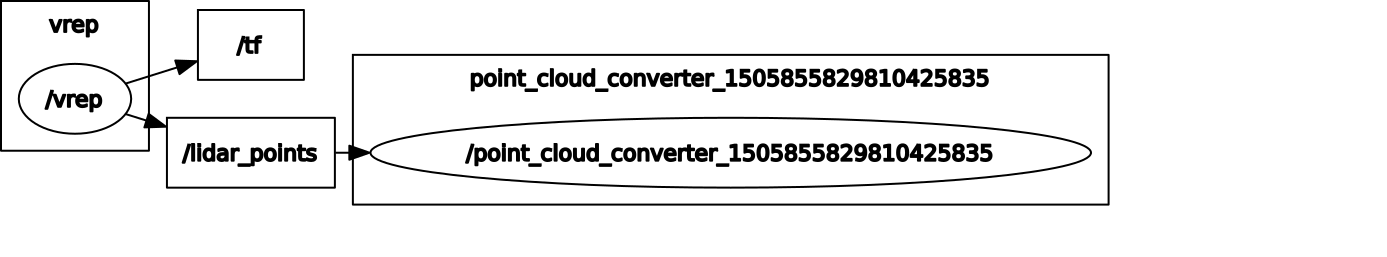
\includegraphics[scale=.22]{index.png} 
  \caption{V-REP as a Node}
\end{figure}
\noindent Above is an example graph for ROS. In the graph VREP is a node wish is publishing the topics tf and lidar\_points. Another node, the point\_cloud\_converter, subscribes to the lidar\_points topic. 
\section{V-REP}
Virtual Robot Experimentation Platform (V-REP) is a platform which allows for robot simulation and control in a 3-D environment. V-REP offers an API and IDE for developement of LUA scripts in customising simulations while also supporting C/C++ plugins. There is also a remote API for V-REP to communicate with other programs. In this project V-REP will be used in conjunction with ROS. To use V-REP with ROS the RosInterface library is used such that V-REP is instantiated as a node in ROS. As a node V-REP will be able to publish transform data and sensor data from the simulation and also be able to subscribe to any topics which might facilitate controls. V-REP also provides for the simulation of a Velodyne VPL-16 LIDAR sensor. Important to note that the lidar sensor is a vision sensor in V-REP and thus utilizes the GPU, with the only other aspect of the simulation which uses GPU being the renderer.  
\section{Simulation Setup}
A Pioneer P3DX is used as the base robot, to which a VPL-16 lidar has been added on to the top platform.  
\begin{figure}[H]
  \centering
  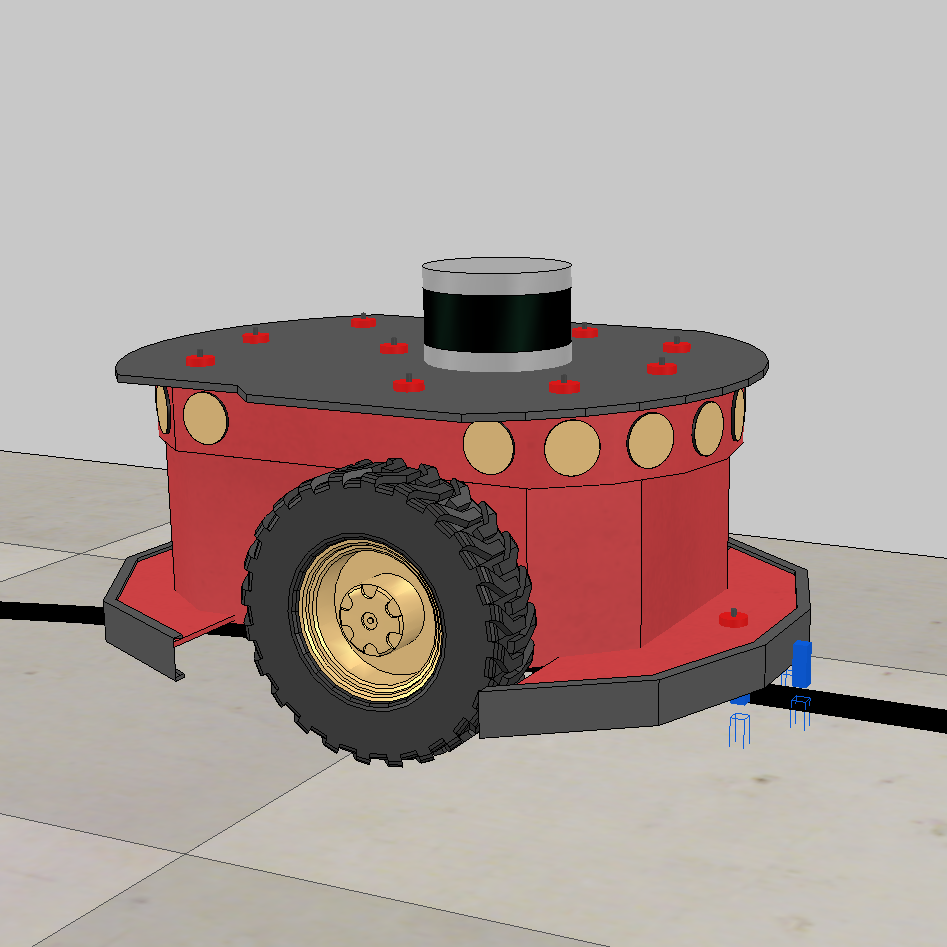
\includegraphics[scale=.15]{robot.png} 
  \caption{Robot in V-REP}
\end{figure}
\noindent This robot begins in a small maze-like environment. In V-REP a basic line following algorithm is implimented using three downward facing vision sensors and a black line on the floor to follow. 
\begin{figure}[H]
  \centering
  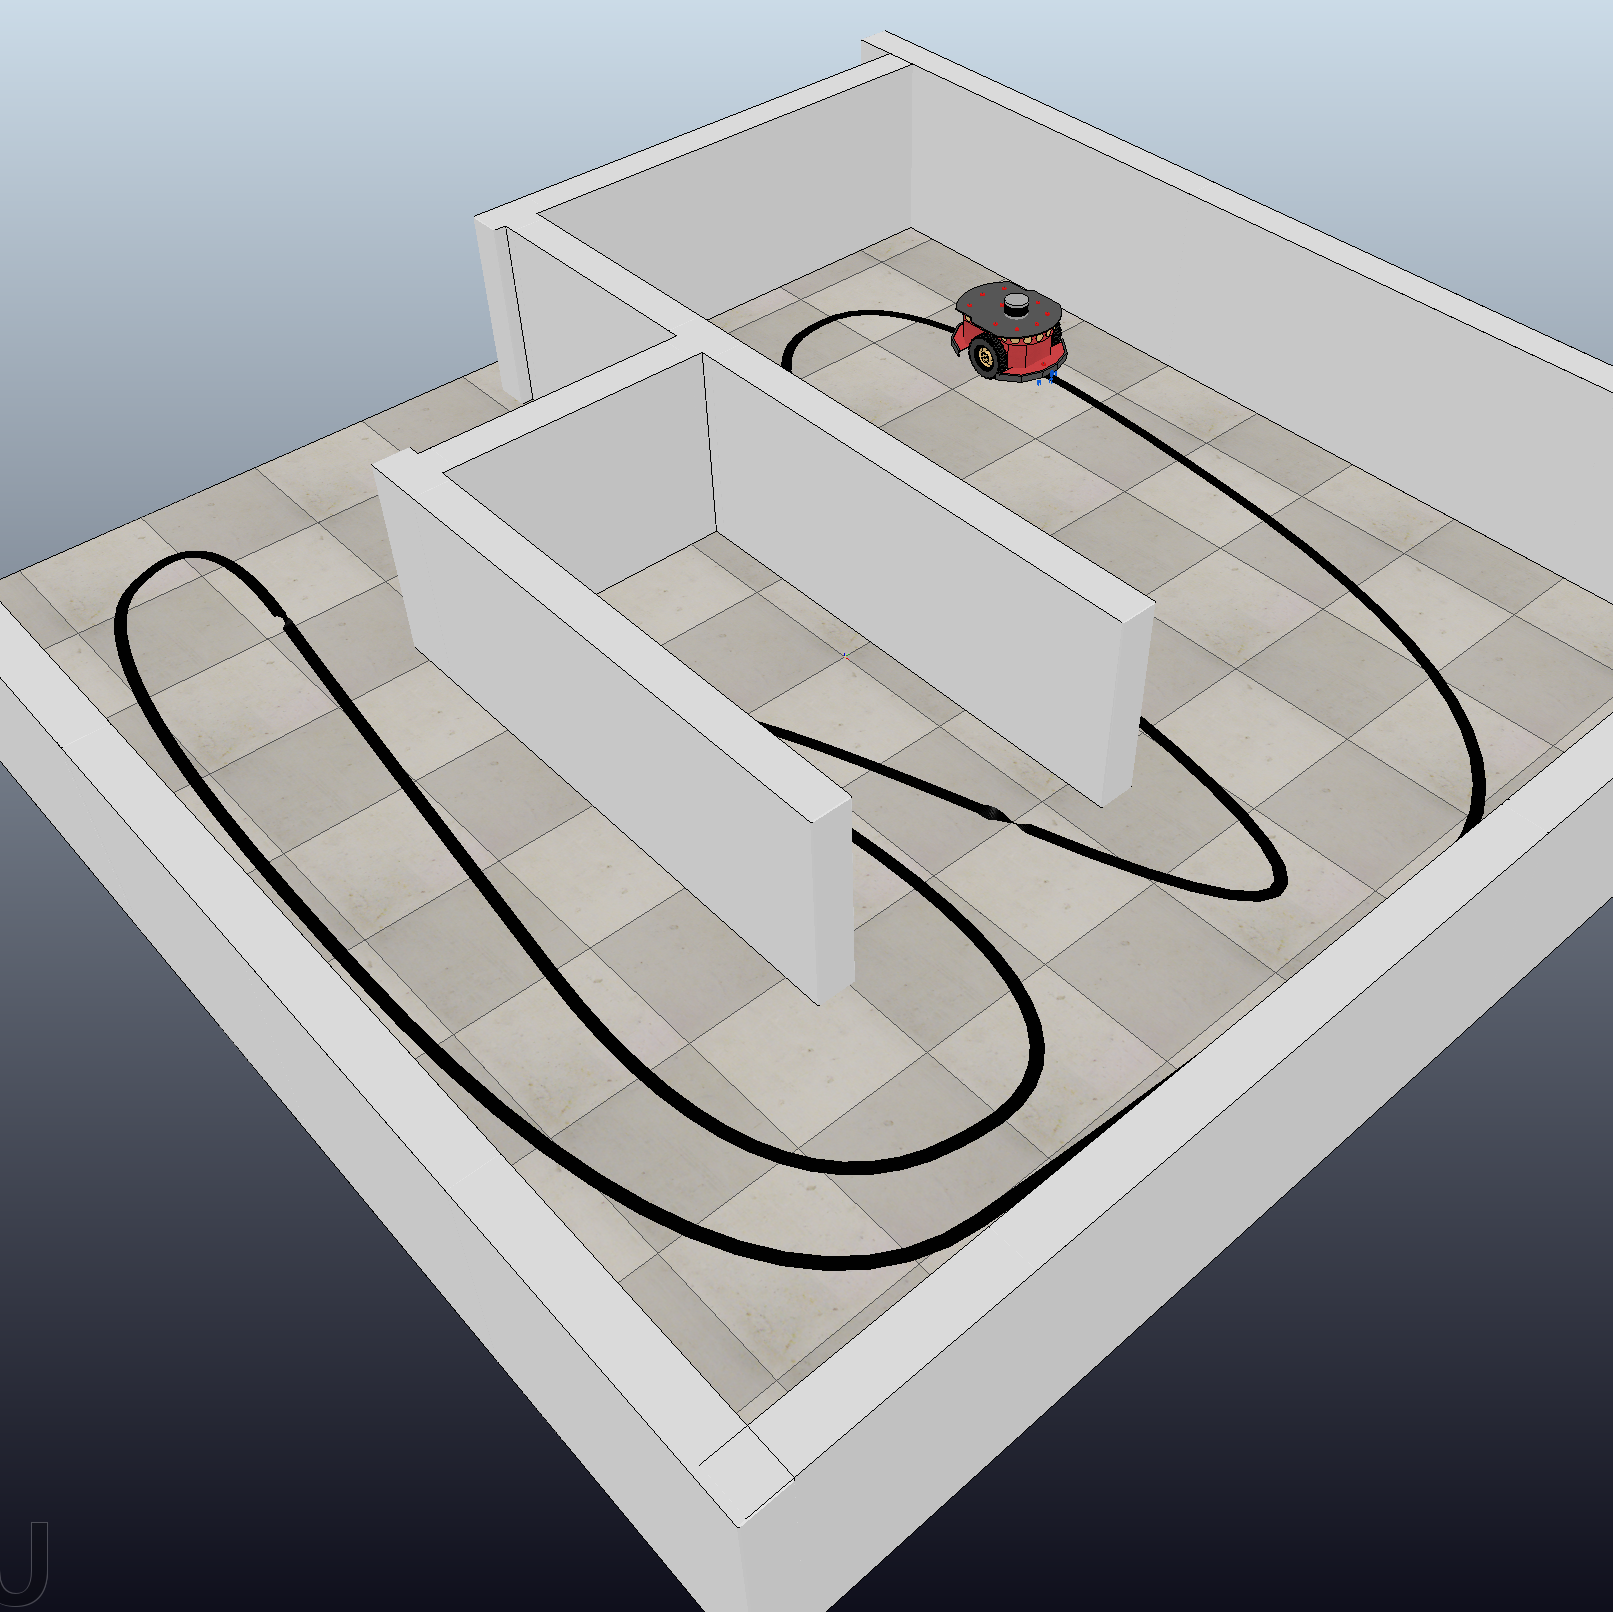
\includegraphics[scale=.1]{maze.png} 
  \caption{Robot in Environment}
\end{figure}
\noindent While the simulation is running it will publish data to two topics. One topic is for the pointcloud data generated by the lidar and the other for the current pose of the robot. The V-REP ROS node will publish these two topics using the rosInterface library. 

\section{SLAM}
Simultaneous Localization and Mapping (SLAM) is a type of algorithm used in robotics for generating maps of a robot's environment and determining the robot's position within that map. Generally a Kalman Filter or Particle Filter is used to provide the estimation of the robot's pose given existing sensor data and the history of observed landmarks or features within the environment.  
\subsection{Feature Extraction}
Feature extraction is how sensor data is converted into usable information. In the case of SLAM feature extraction is how sensor data informs the robot of what surrounds it. An example of feature extraction is a robot with a range sensor sensing a wall and generating a set of points. In this case walls might be identified as lines and the problem would be to extract any lines out of the set of points generated by the range sensor. In this project instead of a typical range sensor a lidar is used to generate the set of points but line extraction is still fine for the simulated environment. 
\section{Appendix}
\subsection{V-REP as a ROS Node}
\indent \indent As a ROS node, V-REP can communicate with other ROS nodes using ROS services, publishers and subscribers. This is accomplished using the RosInterface API provided by Coppelia Robotics. These instructions were created for an Ubuntu 16.04 LTS system running ROS Kinetic and V-REP 3.4.0. 
\\
\indent To setup RosInterface with V-REP 
\begin{enumerate}
\item Download the V-REPs stub generator and install the software it needs. 
\begin{lstlisting}[language=bash,breaklines=true]
sudo apt-get install -y git cmake python-tempita python-catkin-tools python-lxml xsltproc
git clone -q https://github.com/fferri/v_repStubsGen.git
\end{lstlisting}
\item Add path of V-REP stubs generator to the search path of python 
\begin{lstlisting}[language=bash,breaklines=true]
export PYTHONPATH=$PYTHONPATH:$PWD
\end{lstlisting}
\item Create the catkin workspace and initialize it 
\begin{lstlisting}[language=bash,breaklines=true]
mkdir -p ~/project_ws/src
cd ~/project_ws
catkin init
\end{lstlisting}
\item Download RosInterface and build it 
\begin{lstlisting}[language=bash,breaklines=true]
cd src/
git clone --recursive https://github.com/fferri/v_repExtRosInterface.git vrep_ros_interface
catkin build
\end{lstlisting}
\item Source project workspace
\begin{lstlisting}[language=bash,breaklines=true]
source ../devel/setup.bash
\end{lstlisting}
\item Add VREP\_ROOT to the bashrc, assuming it is located in the home folder. Then copy the RosInterface library which was compiled earlier to the V-REP folder.
\begin{lstlisting}[language=bash,breaklines=true]
echo 'export VREP_ROOT="/home/user/V-REP_PRO_EDU_V3_3_2_64_Linux/"' >> ~/.bashrc 
source ~/.bashrc
cp -iv devel/lib/libv_repExtRosInterface.so "$VREP_ROOT/"
\end{lstlisting}
\item Setup alias for v-rep 
\begin{lstlisting}[language=bash,breaklines=true]
echo 'alias vrep="$VREP_ROOT/vrep.sh"' >> ~/.bashrc 
\end{lstlisting}
\item This setup procedure can be validated by running ROS and V-REP, then listing the active ROS nodes. Each command is ran in its own terminal. 
\begin{lstlisting}[language=bash,breaklines=true]
roscore
vrep
rosnode list
\end{lstlisting}
\end{enumerate}
To validate the functionality of the RosInterface the predefined scenes rosInterfaceTopicPublisherAndSubscriber.ttt and controlTypeExamples.ttt can be used. 
\end{multicols*}
 
\end{document}
 
\begin{lstlisting}[language=bash,breaklines=true]
\end{lstlisting}